\chapter{Моделювання термодинамічних процесів у камері. Оцінка параметрів МПД-прискорювача}\label{sec:model_conditions}

\section{Числова модель ТД-розрахунків: комплекс Астра.4}


В основу алгоритму багатоцільовоого програмного комплексу \texttt{Астра.4/рс} покладений універсальний термодинамічний метод визначення характеристик довільних гетерогенних систем, заснований на фундаментальному принципі максимуму ентропії. Цей метод надає можливість узагальненого опису будь-якого високотемпературного стану за допомогою фундаментальних законів термодинаміки, незалежно від умов та способів досягнення стану рівноваги. Метод потребує мінімальної інформації про саму систему та її оточення.

Формулювання задачі ТД-моделювання полягає у призначенні двох умов рівноваги досліджуваної системи з навколишнім середовищем. Ними можуть бути або числові значення ТД-характеристик, або функціональні співвідношення між ними.

Допущення моделі розрахунку у комплексі наступні:
\begin{itemize}
	\item розглядаються системи у стані зовнішньої та внутрішньої термодинамічної рівноваги (повної чи локальної);
	\item розглядаються замкнені системи, тобто такі, що не обмінюються речовиною з навколишнім середовищем;
	\item присутність газової фази є обов'язковим; газова фаза описується рівнянням стану ідеального газу;
	\item поверхневі ефекти на границі поділу фаз не враховуються, розчинність газів у рідкій та твердій фазі відсутня;
	\item конденсовані речовини утворюють однокомпонентні незмішувані фази, або включаються у склад ідеальних конденсованих розчинів.
\end{itemize}

Допускається наявність інших параметрів:
\begin{itemize}
	\item виключення зі складу враховуваних компонентів рівноваги будь-яких індивідуальних речовин;
	\item можливість призначати (фіксувати) концентрації однієї або декількох речовин з подальшим розрахунком рівноваги іншої частини системи;
	\item розгляд неідеальних конденсованих розчинів шляхом введення надлишкової енергії Гіббса;
	\item врахування власного об'єму, що займають конденсовані речовини.	
\end{itemize}

Розрахунки складу фаз та характеристик рівноваги проводяться з використанням внутрішньої бази даних властивостей індивідуальних речовин. База даних є складовою частиною програмного комплексу \texttt{Астра.4/рс}.

Основу інформації у базі даних становлять термодинамічні, теплофізичні та термохімічні властивості індивідуальних речовин, систематизовані у Національному інституті стандартів і технологій США (NIST) та інших ресурсах, опублікованих у відкритих джерелах, обробених розробником комплексу, у тому числі за власними калориметричними та спектроскопічними даними.

У програмному комплексі передбачена можливість введення вихідного складу ТД-систем, утворених дво- та трикомпонентними паливними сумішами за допомогою коефіцієнту надлишку окиснювача та масових часток відповідно. Теоретично необхідне співвідношення компонентів палива, відносно якого задається надлишок окиснювача, обчислюється за допомогою вищих валентностей елементів, що відповідає утворенню повних продуктів згоряння. 

В основному режимі розрахунку параметрів адіабатичного розширення передбачається використання гіпотези локальної термодинамічної рівноваги. Однак можливе проведення обчислень за допомогою різних схем ''заморожування'' складу суміші у соплі.

Програмний комплекс дозволяє виконувати розрахунок ''замороженого'' розширення до заданого тиску, заданого відносного діаметру або ж заданого геометричного ступеня розширення сопла~\cite{Astra}.

Під час розрахунку коефіцієнти втрат питомого імпульсу, втрат в об'ємі камери та соплі для спрощення розрахунку вважались рівними одиниці (розглядається теоретичний випадок поза уточненими експериментально параметрами окремих установок, що можуть індивідуально впливати на ефективність конкретного двигуна).

Процеси впливу електромагнітного поля на потоки іонізуючої присадки та розжарених продуктів згоряння РРД у рамках числової моделі не розглядаються; параметри МПД-прискорювача є результатом оцінки, наведеної у розділі~\ref{sec:model_results}. 

%Модель описує поведінку потоку робочого тіла РРД, враховуючи класичні для такої числової задачі допущення: відсутність в'язкого тертя шарів газу, рух уздовж однієї координатної осі (у нашому випадку вісь абсцис), стисливість за законом ідеального газу (стосується лише взаємодії між частинками самого газу), лагранжева модель дискретної фази для опису руху потоку частинок присадки (металічний дрібнодисперсний калій заданих фракцій з рівномірним розподілом). Задача стаціонарна (програмно використовується опція квазистаціонарності для уточнення розв'язку стаціонарної задачі).

\section{Верифікація моделі. Порівняння з попередніми аналогами}

Для верифікації моделі використовувались технічні параметри існуючого рідинного ракетного двигуна із циклом фазового переходу (expander cycle engine) --- Vinci, що був розроблений у лабораторії DLR Європейського космічного агентства і є одним з найефективніших РРД за показником питомого імпульсу у даний момент~\cite{VinciData}.

У ході попередніх досліджень~\cite{Previous} для побудови аналогічної моделі поведінки потоку робочого тіла у двигуні застосовувався програмний пакет \texttt{ANSYS} Student 2021R1 (підпроцесор Fluent), результати роботи якої було порівняно з розрахунком у пакеті \texttt{Астра.4/рс}.

Основні параметри моделі-аналога:

\begin{itemize}
	\item тип розрахункової моделі - PBСS (Pressure-based Coupled Solver);
	\item чисельно розв'язувалась система рівнянь Ейлера для стисливого газу (нерозривності, збереження імпульсу та збереження енергії)~\cite{GuidePBCS};
	\item задача симетрична відносно осі камери і сопла, була задана кінетична схема горіння пального в окиснювачі (водень/кисень);
	\item модель турбулентності $k-\varepsilon$ з розрахунком релаксаційного множника для турбулентної в'язкості (т. зв. схема Realizable $k-\varepsilon$)~\cite{GuideKEpsilon} із застосуванням методу Finite-Rate/Eddy-Dissipation для уточнення впливу турбулентних течій на кінетику реакцій у КЗ~\cite{GuideChemistry};
	\item застосована радіаційна модель Rosseland із заданим параметром матеріалу стінки та її товщиною~\cite{GuideRosseland};
	\item для моделювання руху частинок присадки застосовується лагранжева модель дискретної фази (DPM) з урахуванням теплообміну між газом та частинками~\cite{GuideDPM}.
\end{itemize}

Граничні умови задані на вході у камеру згоряння (масова витрата палива, а також температура подачі компонентів, зазначена у документації~\cite{VinciDataDLR} - 250 K) і на виході з розрахункової області, зовнішній тиск відповідно до середовища роботи даного РРД становить $50$~мбар ($5$~кПа), температура 293~K.

Товщина стінки камери й сопла - $20$~мм. Матеріал --- алюміній, наявний у переліку матеріалів солвера, коефіцієнти поглинання задані за умовчанням.

Додатково у попередній CFD-моделі було проведене моделювання за присутності присадки калію для визначення оптимального розміру частинок за визначеної масової частки у робочому тілі двигуна.

Умови для потоку присадки - металічний дрібнодисперсний калій з заданими значеннями густини $ 856 $~кг/м$^3$ і теплоємності $871$~Дж/(кг $\cdot$ К); подача присадки здійснюється з входу в камеру згоряння поряд з паливними компонентами, температура 300 K, швидкість подачі взята аналогічною швидкості потоку палива на вході ($118$ м/с ; розраховується автоматично процесором після задання граничних параметрів). Задана витрата становить 0.397 кг/с, що становить 0.01 витрати робочого тіла установки (характерне значення, використовуване в МПД-прискорювачах, згідно даних~\cite{Panchenko}).

\begin{figure}
	\centering
	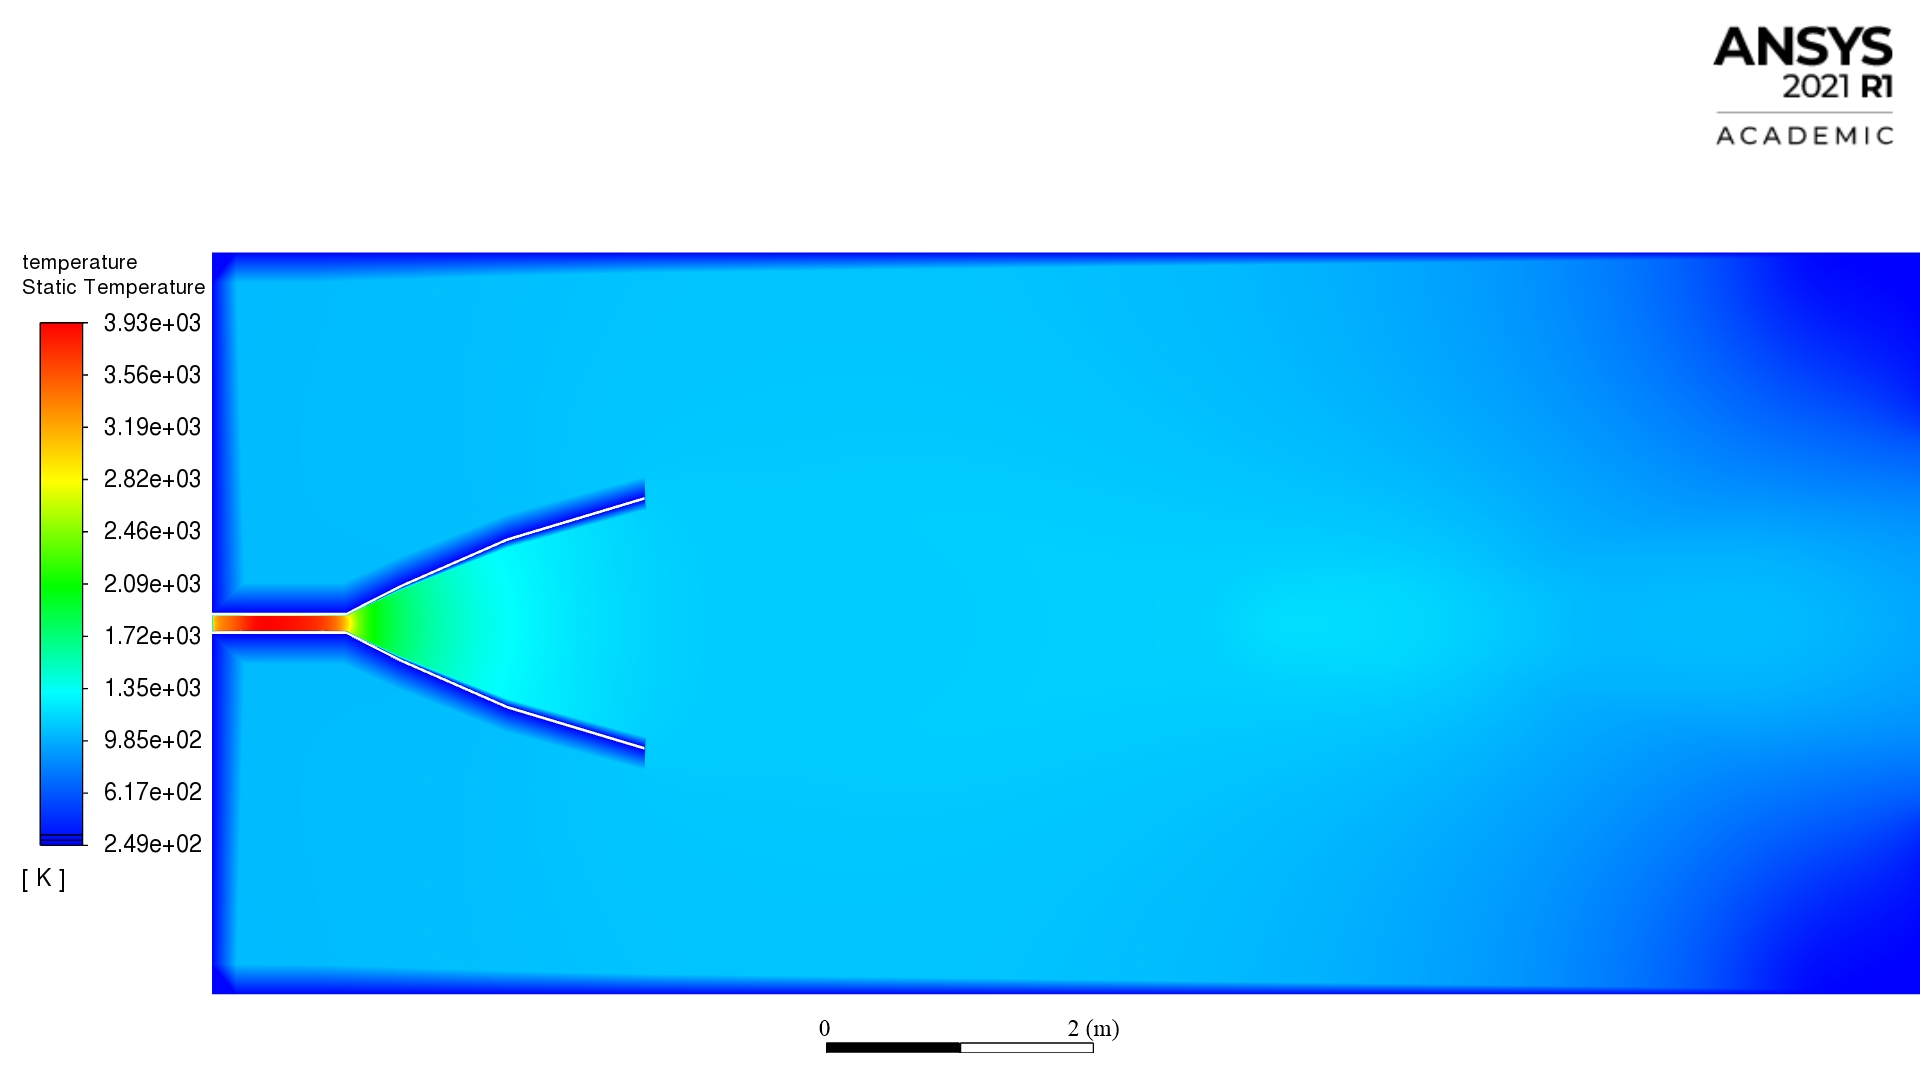
\includegraphics[width=0.7\textheight, angle=0,origin=c]{chapter_3/pure_temperature.jpg}
	\caption{Поле температур (розрахунок без введення присадки, CFD-модель з попереднього дослідження)~\cite{Previous}}
	\label{fig:pure_temperature}
\end{figure}

Верифікація здійснювалась шляхом порівняння тиску та температури у камері, розрахованих у пакеті Fluent (рис.~\ref{fig:pure_temperature}), з отриманими значеннями з розрахунку у пакеті \texttt{Астра.4/рс} (рис.~\ref{fig:Vinci_1perc_pure}) і фактичними значеннями характеристик двигуна. Результати верифікації наведені у табл.~\ref{tab_verification}.

\begin{figure}
	\centering
	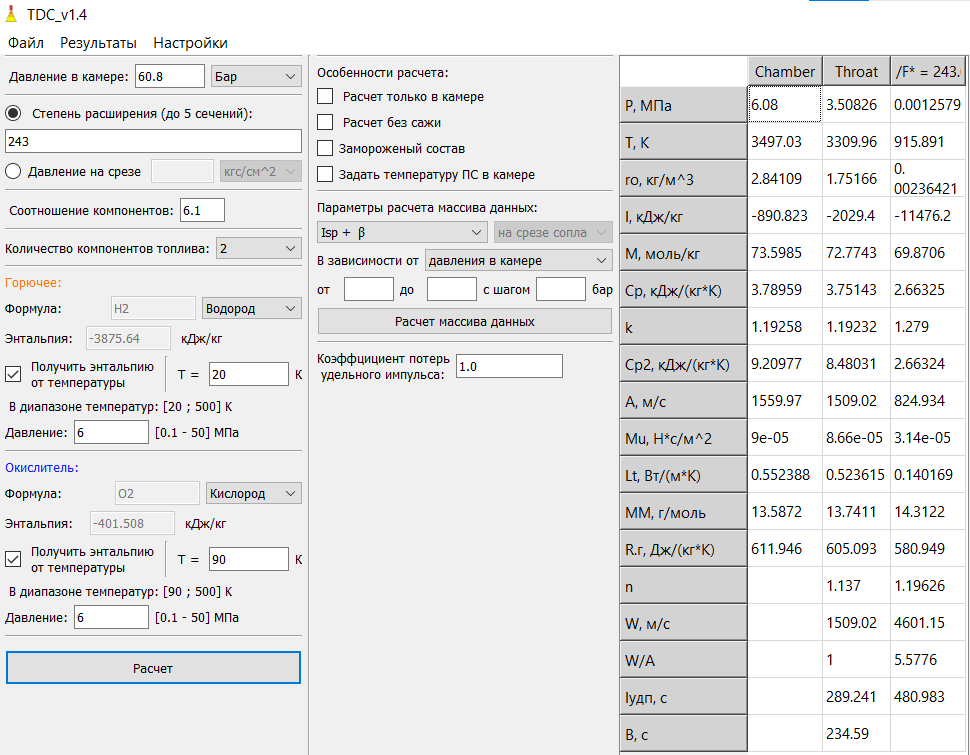
\includegraphics[width=0.7\textheight, angle=0,origin=c]{chapter_2/Vinci_1perc_pure.png}
	\caption{Розрахунок термо- і газодинамічних параметрів камери двигуна ESA Vinci (інтерфейс оболонки програмного комплексу Астра.4/рс )}
	\label{fig:Vinci_1perc_pure}
\end{figure}

\begin{table}[t!]\centering\small
	\caption{Результати верифікації моделі розрахунку у комплексі \texttt{Астра.4/рс} відносно фактичних характеристик РРД ESA Vinci~\cite{VinciData}~\cite{VinciDataDLR} і CFD-моделі \texttt{ANSYS} Fluent}
	\begin{tabular}{|l|c|c|c|c|}
		\hline
		\thead{} & \thead{Література} & \thead{Fluent} & \thead{Астра.4}\\
		\hline
		Тиск у камері, бар & $60.8$ & $80$ & $60.8$\\
		\hline
		Температура у камері, К & $3600$ & $3930$ & $3497$ \\
		\hline
		Відхилення показника тиску, \% & -- & $31.58$ & -- \\
		\hline
		Відхилення температури, \% & -- & $9.17$ & $2.86$ \\		
		\hline
	\end{tabular}
	\label{tab_verification}
\end{table}	


\section{Постановка умов задачі. Розрахунки на основі параметрів існуючих РРД}


Для додаткової верифікації моделі (порівняння з фактичними параметрами існуючих РРД) були розраховані термодинамічні параметри (без додавання присадки) камер декількох ракетних двигунів різних діапазонів потужностей - від кількох тонн (Flight Control SV3, 3 тс) до великих установок для важких ракет-носіїв (РД-120, 85 тс; РД-0120, 200 тс), що можуть бути потенційно застосовані у складі плазморідинного двигуна. За результатами, теоретичні розрахункові параметри РРД, зокрема тяга, питомий імпульс і витратний комплекс (без урахування коефіцієнтів реальних втрат камери, сопла та ін.) відповідають їх характеристикам.

Після верифікації у цьому ж пакеті (застосовуючи ідентичні моделі кінетики взаємодії компонентів) були проведені розрахунки за присутності визначеної масової частки присадки робочого тіла МПД-прискорювача, що складала 2\% від витрати двигуна. За результатами двох розрахунків (камера без присадки і за її присутності) визначався спад параметрів камери РРД. Отримані значення наведені у розділі~\ref{sec:model_results} (табл.~\ref{tab_LPRE}).

%Побудова геометрії задачі здійснена з урахуванням потреби в оптимізації розрахункової області для отримання високої точності розрахунку на доступних обчислювальних потужностях. Оптимальним у такому випадку виявляється 2D~-~вісесиметричний профіль, що і був побудований в окремій програмі та імпортований в пакет \texttt{ANSYS}. Геометричні параметри взяті з технічної документації згаданого РРД $Vinci$ \cite{VinciData}.
%Розрахункова геометрія побудована у $SolidWorks$ $2020$, її вигляд наведено на рис.~\ref{fig:geometry_advanced_screen_new}.



%Розрахункова сітка побудована засобами препроцесора \texttt{ANSYS} $Meshing$; вихідний варіант містить 107562 комірок і 105066 вузлів з основним адаптивним та додатковим локальним розбиттям у ділянках, де потребується згущення (камера згоряння, критичний переріз сопла, область за зрізом стінки і зрізом сопла далі по довжині розрахункової області). Розміри елементів (довжини сторін чотирикутних комірок) в залежності від локального розбиття варіюються від $50$ мкм (критика сопла) до $5$ мм; ділянки обабіч сопла розташовані поза потоком, сітка у них має менше згущення.


\section{Параметри робочого тіла МПД-прискорювача}

 
\begin{figure}[h!]
	\centering
	\subfloat[$5$ мкм]{%
		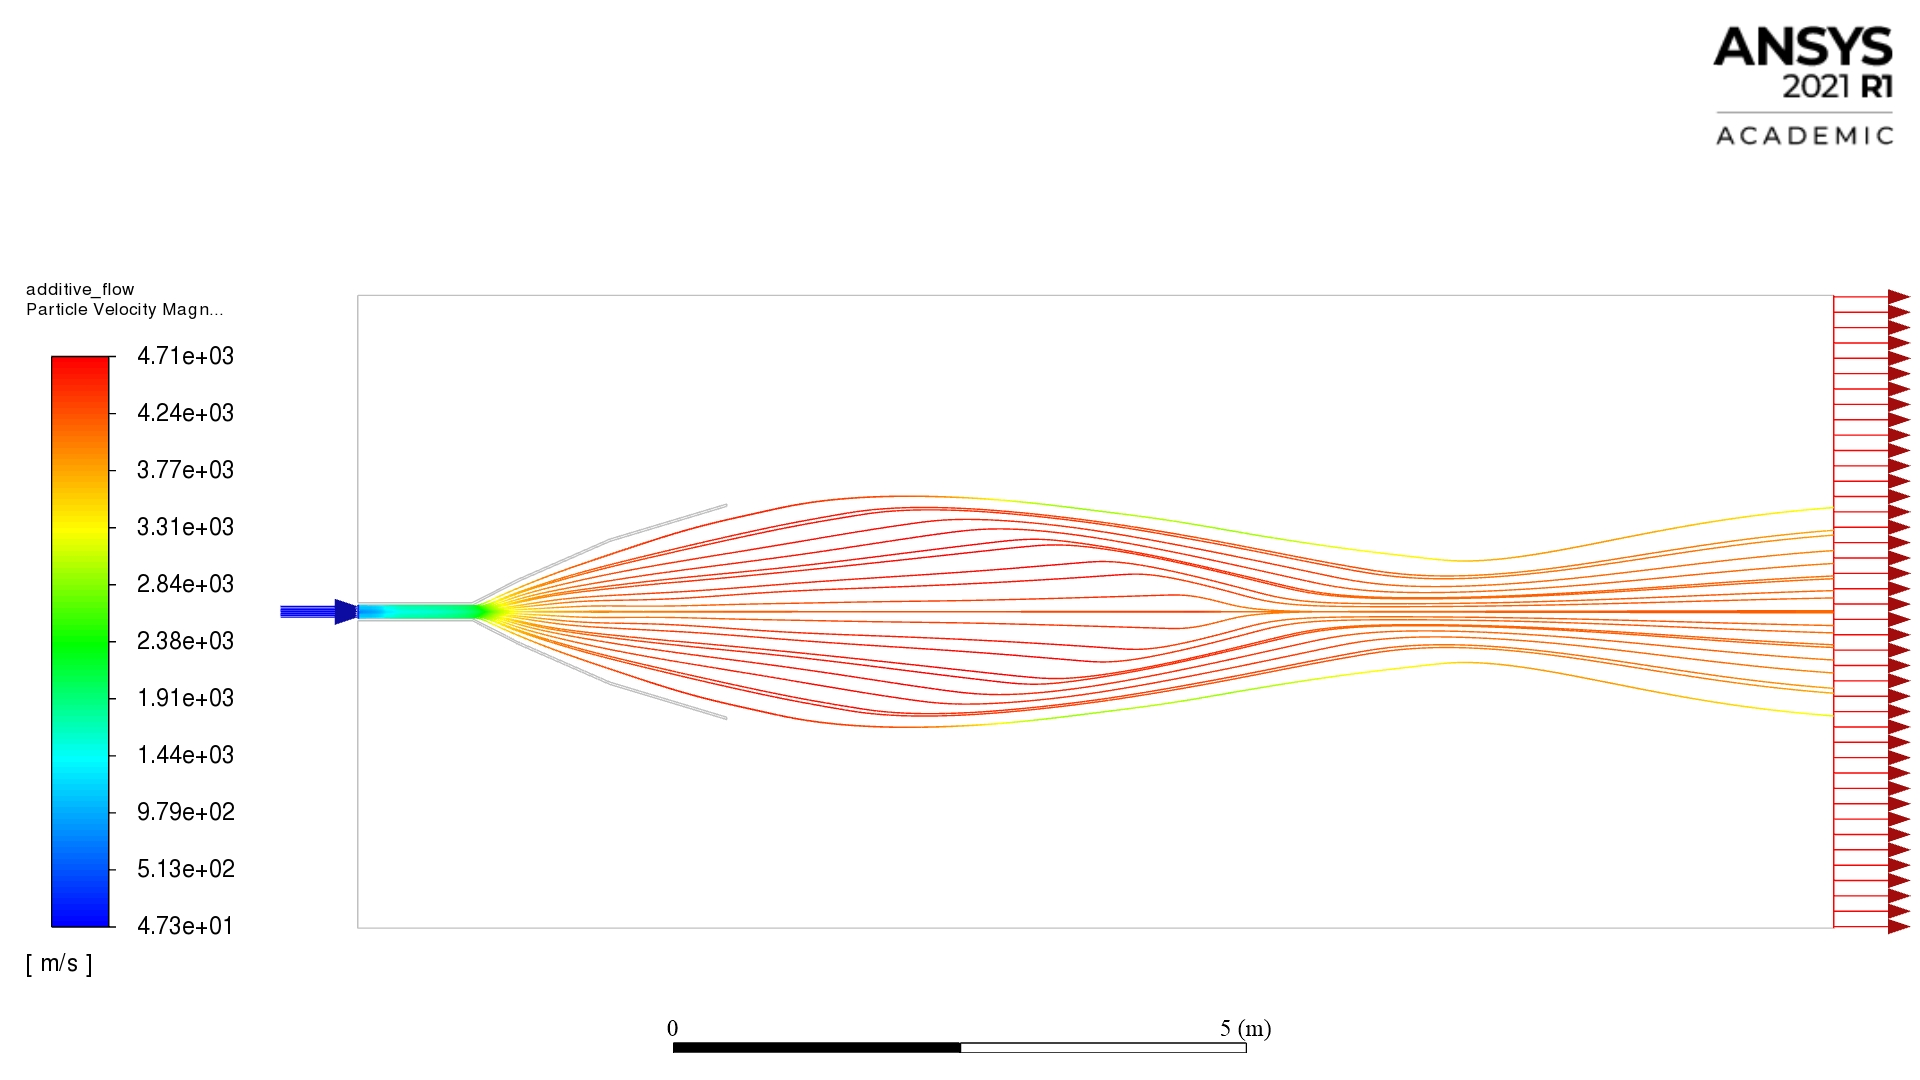
\includegraphics[width=0.4\columnwidth]{chapter_3/additive_5.jpg}
		\label{subfig1}
	}%
	\\ % <- для того, щоб рисунки розташувались в колонку
	\subfloat[$10$ мкм]{
		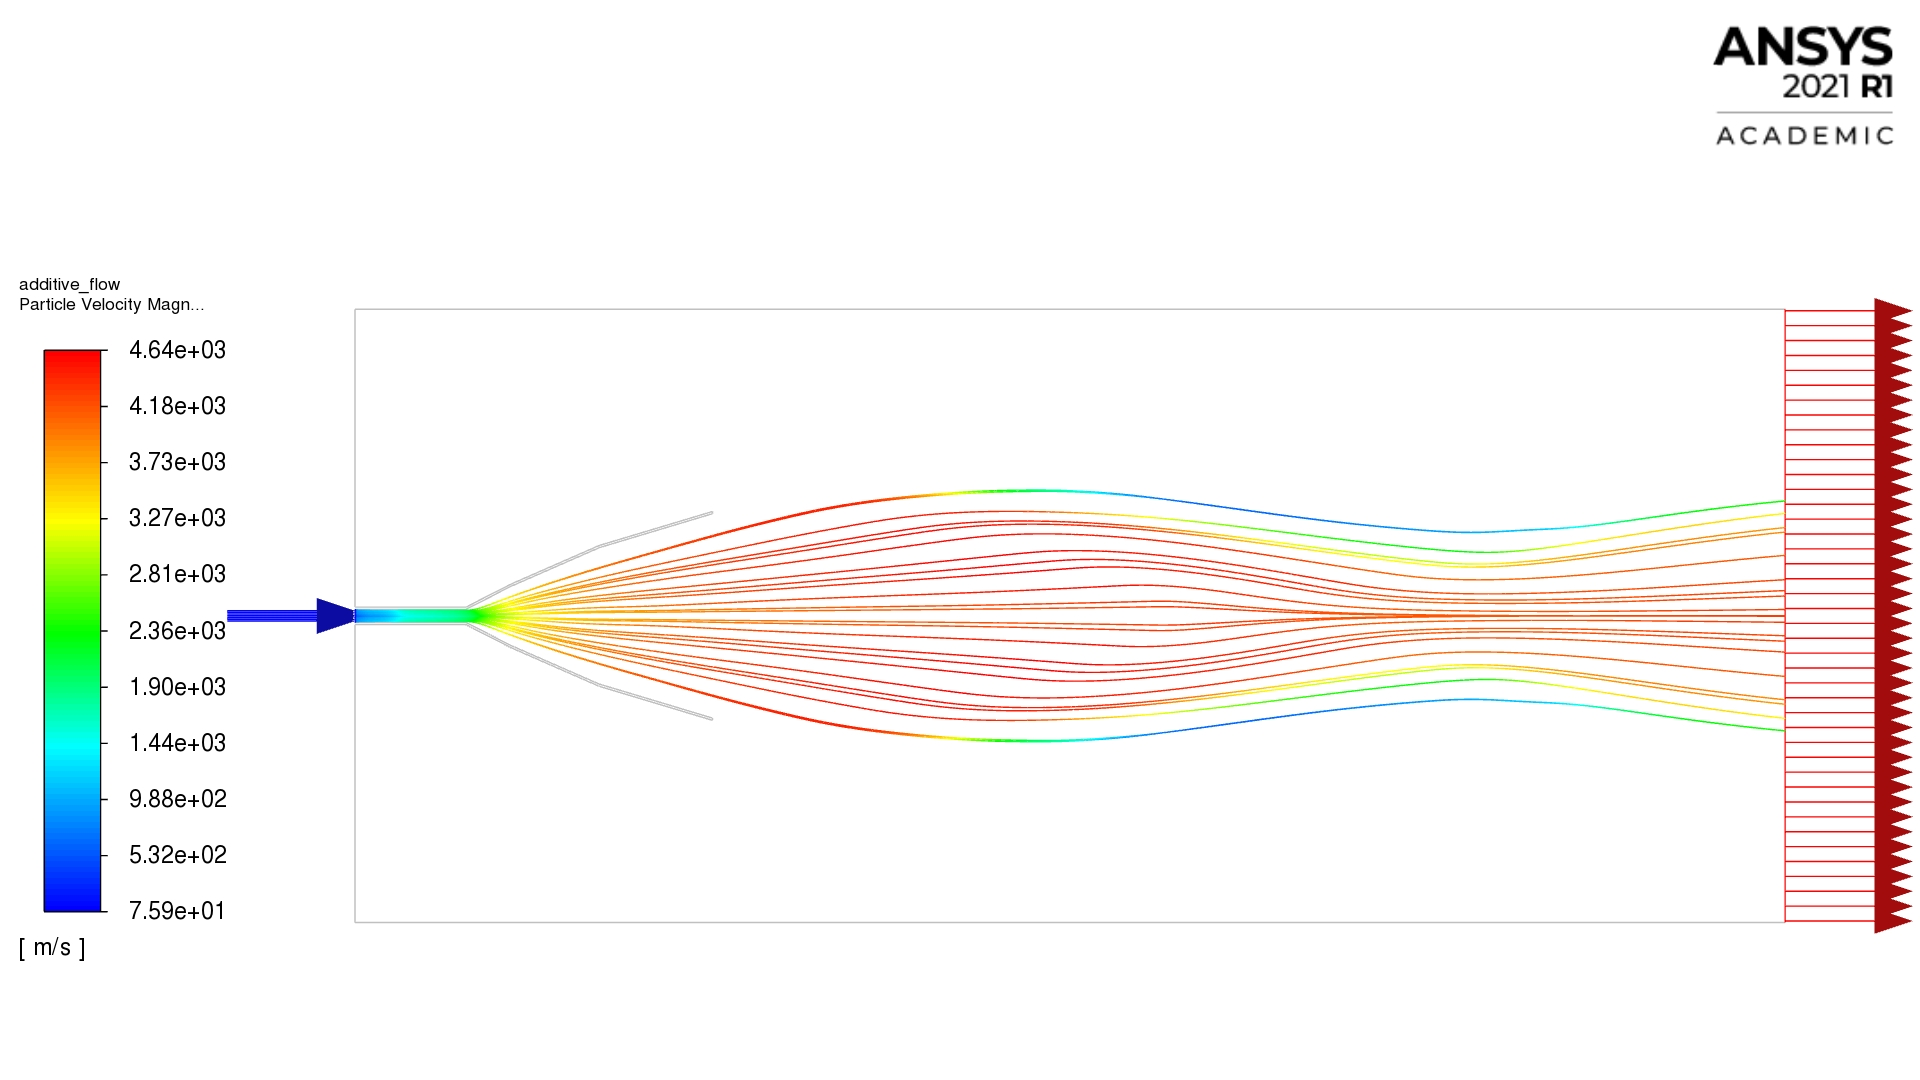
\includegraphics[width=0.4\columnwidth]{chapter_3/additive_10.jpg}
		\label{subfig2}
	}%
	% <- для того, щоб рисунки розташувались в колонку
	\subfloat[$20$ мкм]{
		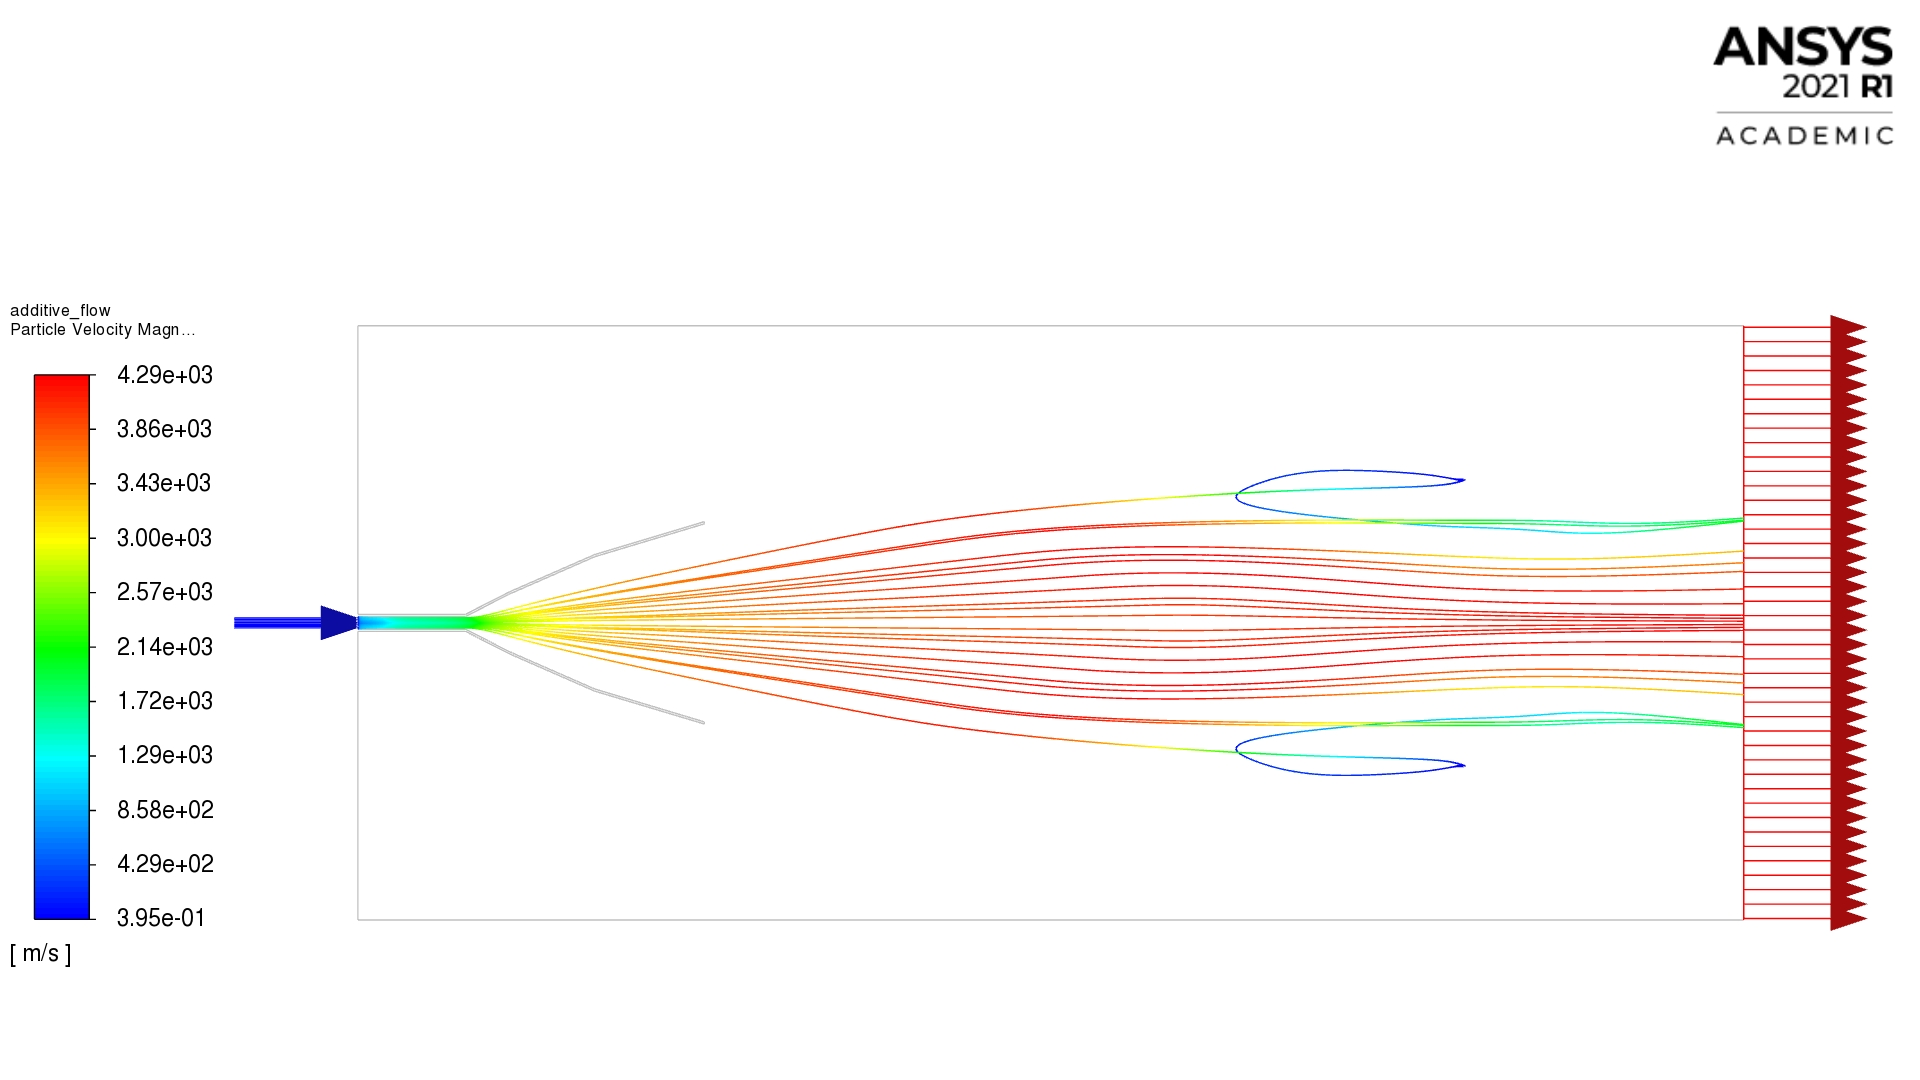
\includegraphics[width=0.4\columnwidth]{chapter_3/additive_20.jpg}
		\label{subfig3}
	}%
	\\ % <- для того, щоб рисунки розташувались в колонку
	\subfloat[$50$ мкм]{
		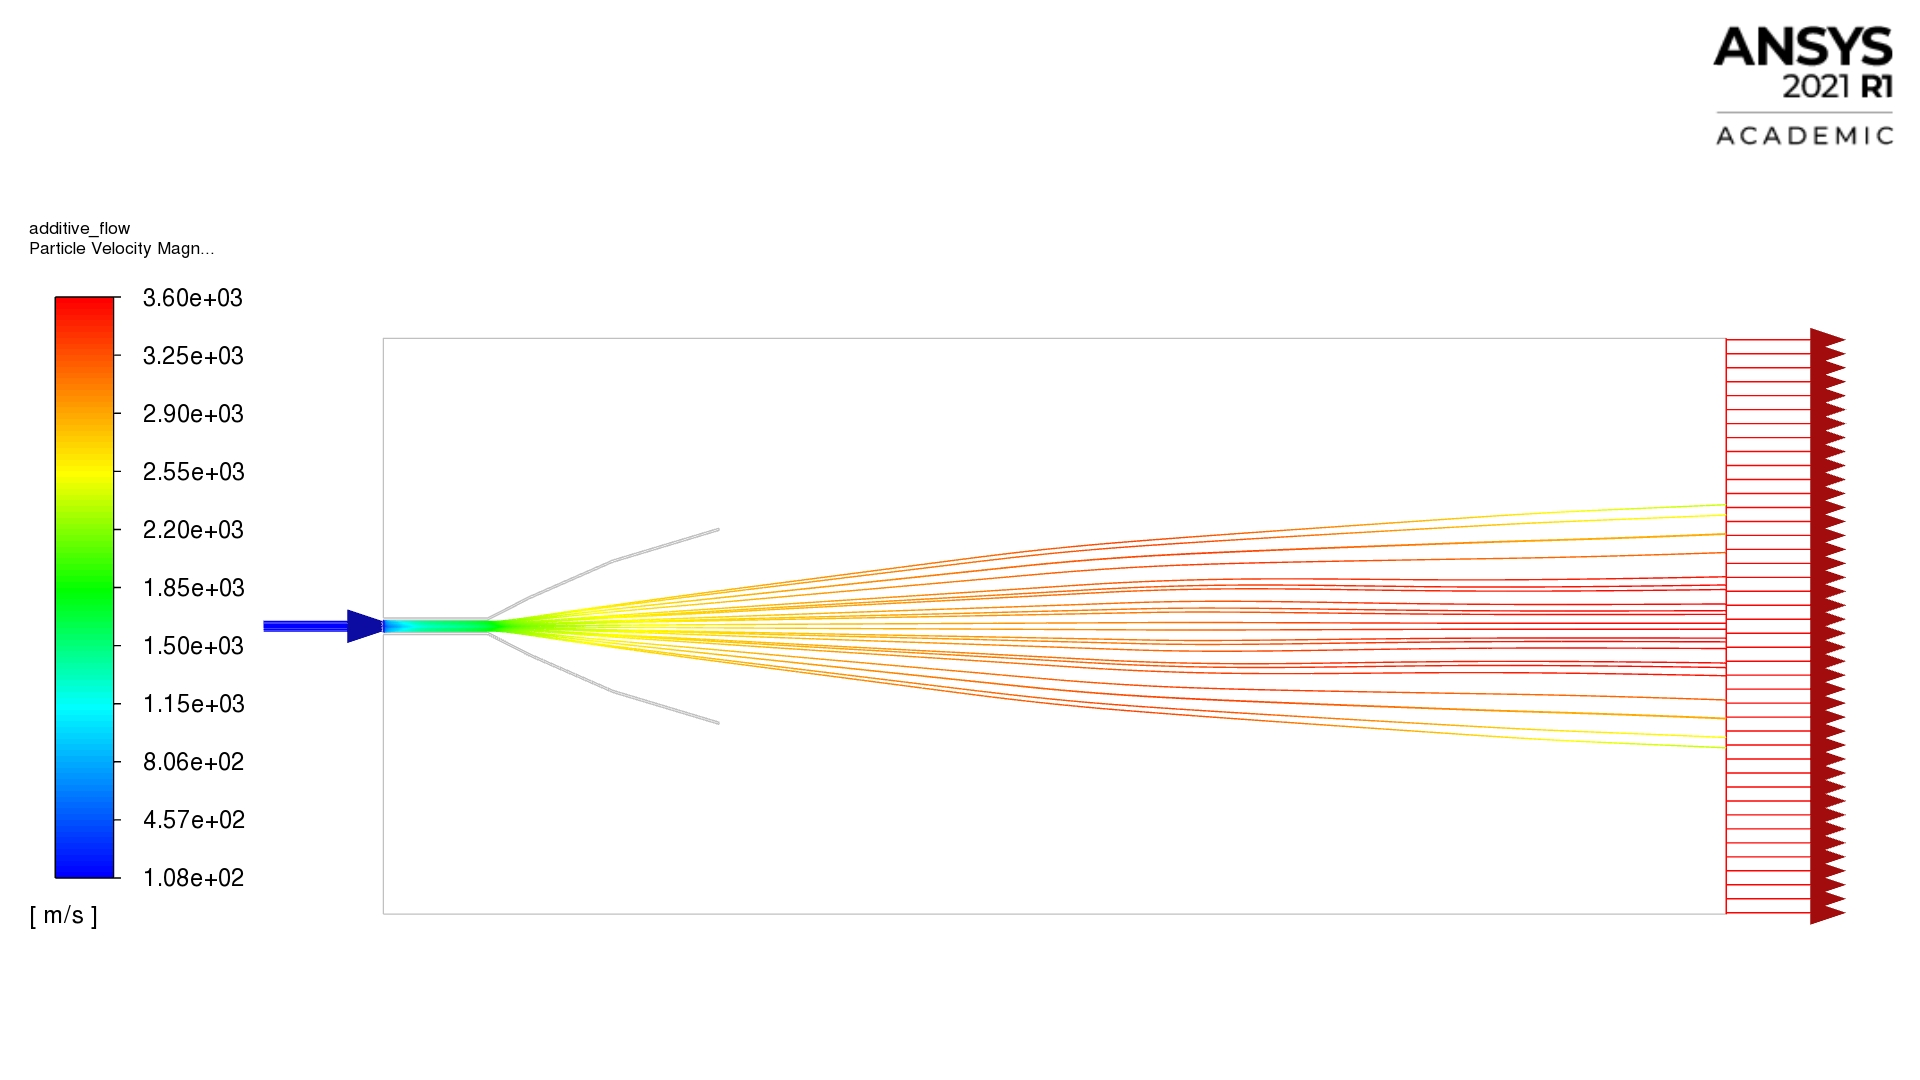
\includegraphics[width=0.4\columnwidth]{chapter_3/additive_50.jpg}
		\label{subfig4}
	}%
	% <- для того, щоб рисунки розташувались в колонку
	\subfloat[$75$ мкм]{
		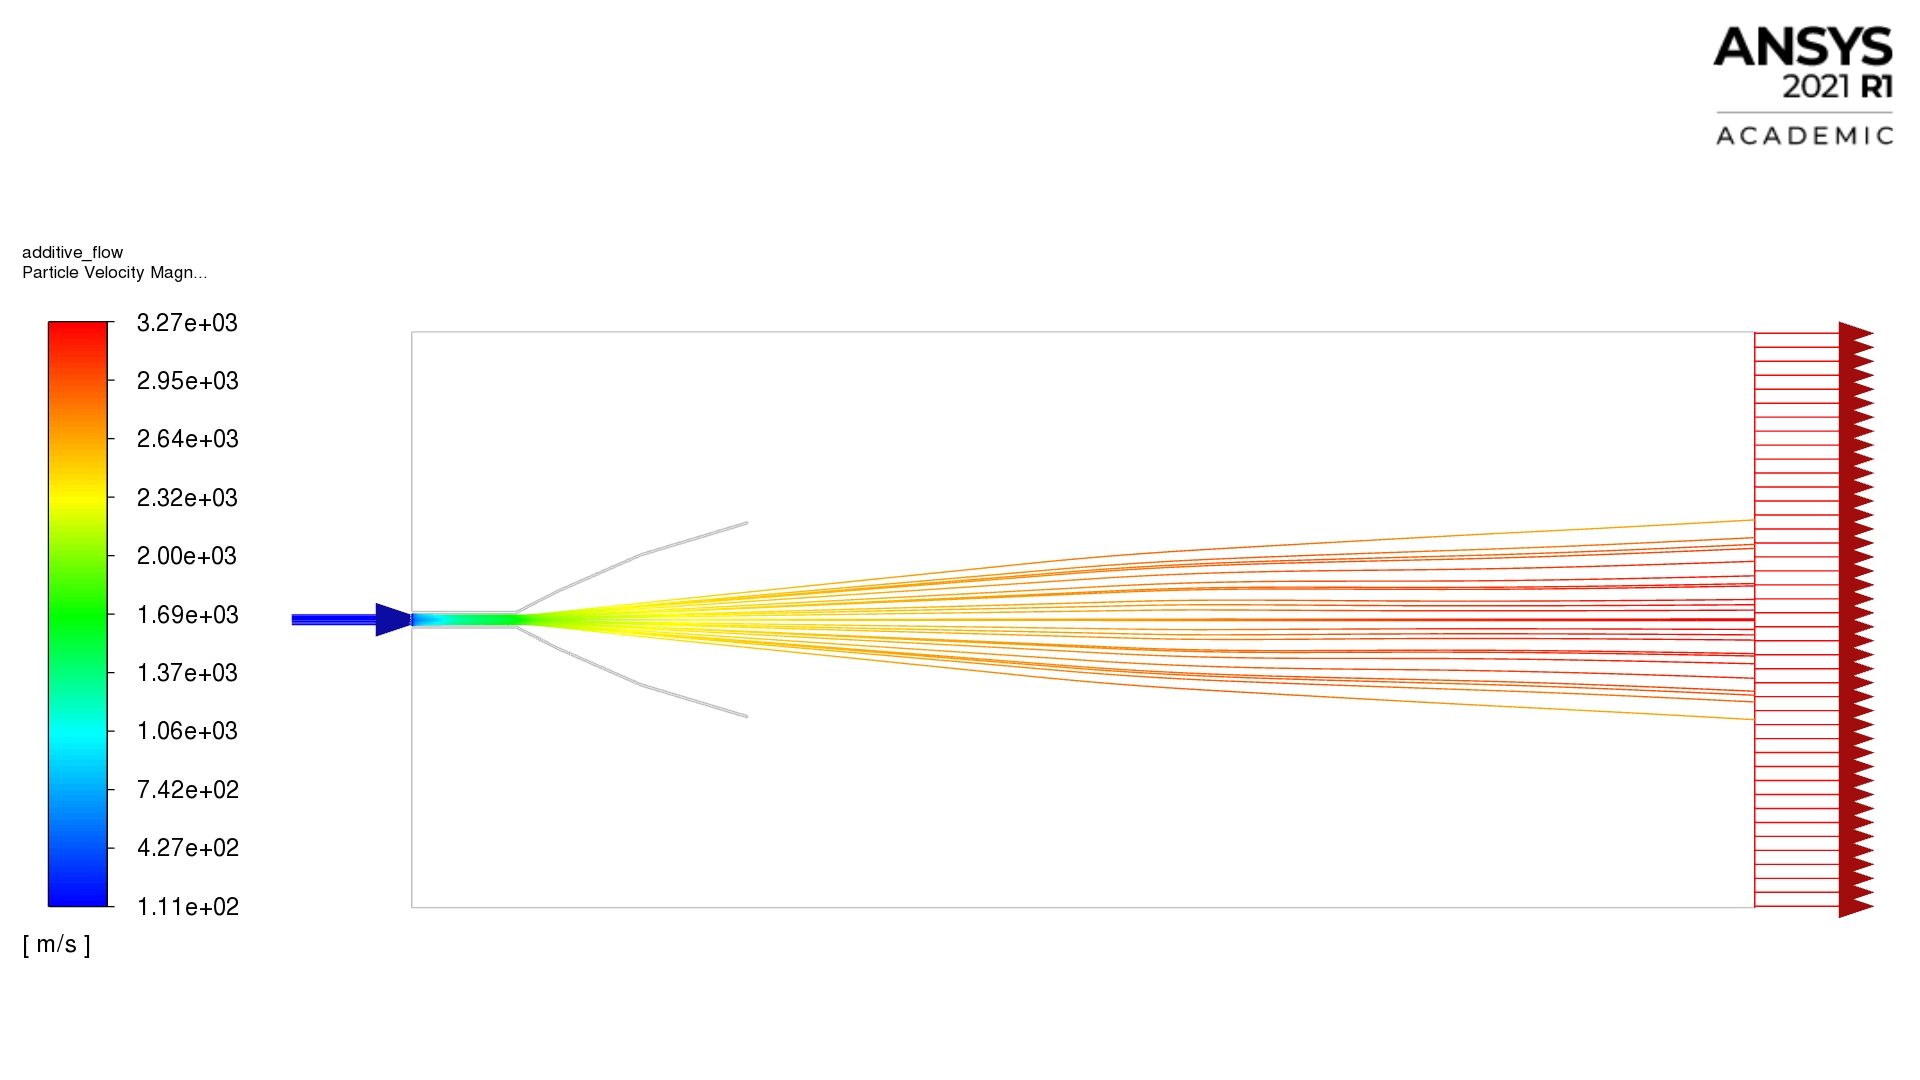
\includegraphics[width=0.4\columnwidth]{chapter_3/additive_75.jpg}
		\label{subfig5}
	}%
	\\
	\caption{Траєкторії частинок присадки калію різних фракцій, введеної в РРД (CFD-модель з попереднього дослідження)~\cite{Previous}}
\end{figure}

У якості робочого тіла МПД-прискорювач використовує дрібнодисперсний порошок калію; подача присадки має здійснюватись з окремої форсунки паралельно з паливними компонентами. Оптимальний розмір частинок був визначений у попередньому дослідженні~\cite{Previous}; спираючись на результати CFD-моделювання, для забезпечення належного прогріву частинок у потоці газу (максимізації температури присадки на виході з камери) і водночас мінімізації можливих процесів ерозії стінки КЗ і сопла розмір частинок присадки доцільно брати рівним 10 мкм (див. рис.~\ref{subfig2}). Для збільшення питомої тяги електроракетної установки частка присадки збільшена до 2\% (0.02 витрати робочого тіла установки; характерне значення, використовуване в МПД-прискорювачах, згідно даних~\cite{Panchenko}, становить від 1 до 10\% для МГД-установок на присадках лужних металів).

\section{Висновки розділу 2}

Для належної точності числового моделювання необхідно застосувати програмний комплекс, що включає у себе моделі поведінки паливних компонентів за умов камери згоряння РРД. Такий комплекс було підібрано, проведена верифікація згідно відомих енергетичних параметрів декількох типів існуючих РРД; було проведене порівняння з CFD -- моделлю для аналогічних розрахунків, виконаною у попередньому дослідженні.

Задача термодинамічного моделювання поведінки паливних сумішей є апробованою, проте має певні особливості (високі значення тисків та температур, наявність активних процесів рекомбінації тощо), що враховуються застосованим програмним комплексом.

Побудована і верифікована відносно параметрів існуючих двигунів модель дозволяє виводити усі основні необхідні параметри енергетичного розрахунку РРД.

Параметри двигунів були опрацьовані вищеозначеним програмним комплексом \texttt{Астра.4/рс}, здійснене моделювання термодинаміки КЗ трьох різних двигунів, проведений їх енергетичний розрахунок.   